\documentclass[12pt]{article}
\usepackage[a4paper, margin=.30in]{geometry}
%\usepackage{array}
\usepackage{pgfplots}
\pgfplotsset{compat=1.18} % Version de PGFPlots
\usepackage{array}
\usepackage{fancybox}
\usepackage{amsmath,amsfonts,amssymb}
\usepackage{graphicx}
\usepackage{array}
\usepackage{booktabs}
\usepackage{xcolor}
\usepackage{multirow}
\usepackage{tikz}
\usepackage{float}
\usepackage{hyperref}
\usepackage{subfig, wrapfig, makecell}
\usepackage{pgf-pie}

\newcommand\headerMe[2]{\noindent{}#1\hfill#2}
\renewcommand \thesection{\Roman{section}}

\newcolumntype{M}[1]{>{\raggedright}m{#1}}




\begin{document}

\headerMe{Royaume du Maroc}{année scolaire \emph{2024-2025}}\\
\headerMe{Ministère de l'Éducation nationale, }{  Professeur :\emph{Zakaria Haouzan}}\\
\headerMe{du Préscolaire et des Sports}{Établissement : \emph{Lycée SKHOR qualifiant}}\\

\begin{center}
Devoir surveillé N°2-S1 \\
Durée 2h00\\
\underline{2-BAC Section des sciences Mathématiques}\\

    \vspace{.2cm}
\hrulefill
\Large{Fiche Pédagogique}
\hrulefill\\
\end{center}
%end Headerss------------------------


%__________________Chimie ______________________-
%%%%%%%+_+_+_+_+_+_+_+_+_Partie1
\section[A]{Introduction }
\hspace{0.5cm}Le programme d'études de la matière physique chimie vise à croître un ensemble de compétences visant à développer la personnalité de l'apprenant. Ces compétences peuvent être classées en Compétences transversales communes et Compétences qualitatives associées aux différentes parties du programme.
\section{cadre de référence }
 \hspace{0.5cm}L'épreuve a été réalisée en adoptant des modes proches à des situations d'apprentissages et des situations problèmes, qui permettent de compléter les connaissances et les compétences contenues dans les instructions pédagogiques et dans le programme de la matière physique chimie et aussi dans le cadre de référence de l'examen national. 
 \\Tout en respectant les rapports d'importance précisés dans les tableaux suivants :
 \begin{center}
\begin{tabular}{|c||c||c|}
\hline
    \textbf{Restitution des Connaissances} & \textbf{Application des Connaissances} & \textbf{Situation Problème }\\
    \hline 
    $40\%$ & $30\%$ & $30\%$\\
    \hline
\end{tabular} 
\end{center}

\section{tableau de spécification}

\begin{center}
\begin{tabular}{|p{3.5cm}|p{3.5cm}|p{3.5cm}|p{3.5cm}|p{1.5cm}|}
\hline
\textbf{Niveau d'habileté} & \textbf{Restitution des Connaissances} & \textbf{Application des Connaissances} & \textbf{Situation Problème} & \textbf{La somme} \\
\hline
\multirow{3}{*}{\textbf{Les Ondes 53\%}} & & & & \multirow{3}{*}{\textbf{53\% 13pts 12Q 65min}} \\
\cline{1-1}
Les Ondes mécaniques progressives & 5\% 1Q - 0,5pts & 4\% 1Q - 1pts & 4\% 1Q - 1pts & \\
\cline{1-4}
Les Ondes périodiques & 8\% 2Q - 1pts & 6\% 1Q - 1,5pts & 6\% 1Q - 1,5pts & \\
\cline{1-4}
Les Ondes lumineuses & 8\% 3Q - 2pts & 6\% 3Q - 2pts & 6\% 1Q - 2,5pts & \\
\hline
\multirow{2}{*}{\textbf{Les Transformations d'un système chimique 47\%}} & & & & \multirow{2}{*}{\textbf{47\% 7pts 10Q 55min}} \\
\cline{1-1}
Lentes et rapides & 4\% 2Q - 1pts & 3\% 1Q - 0,5pts & 3\% 1Q - 0,5pts & \\
\cline{1-4}
Suivi temporel & 15\% 2Q - 1,5pts & 11\% 2Q - 2pts & 11\% 2Q - 1,5pts & \\
\hline
\textbf{Total} & \textbf{40\% 10Q - 6pts} & \textbf{30\% 8Q - 7pts} & \textbf{30\% 6Q - 7pts} & \textbf{100\% 20pts} \\
\hline
\end{tabular}
\end{center}

\section{Analyse Statistique des Résultats}

\subsection{Distribution des Notes}
L'analyse porte sur un effectif de 7 élèves ayant passé l'examen. Voici les principales statistiques concernant les résultats obtenus:

\begin{center}
\begin{tabular}{|l|c|}
\hline
\textbf{Statistique} & \textbf{Valeur} \\
\hline
Note minimale & 5,75 /20 \\
Note maximale & 17,00 /20 \\
Moyenne de la classe & 11,64 /20 \\
Médiane & 12,25 /20 \\
Écart-type & 4,16 \\
\hline
\end{tabular}
\end{center}

\subsection{Visualisation de la Distribution}

\begin{center}
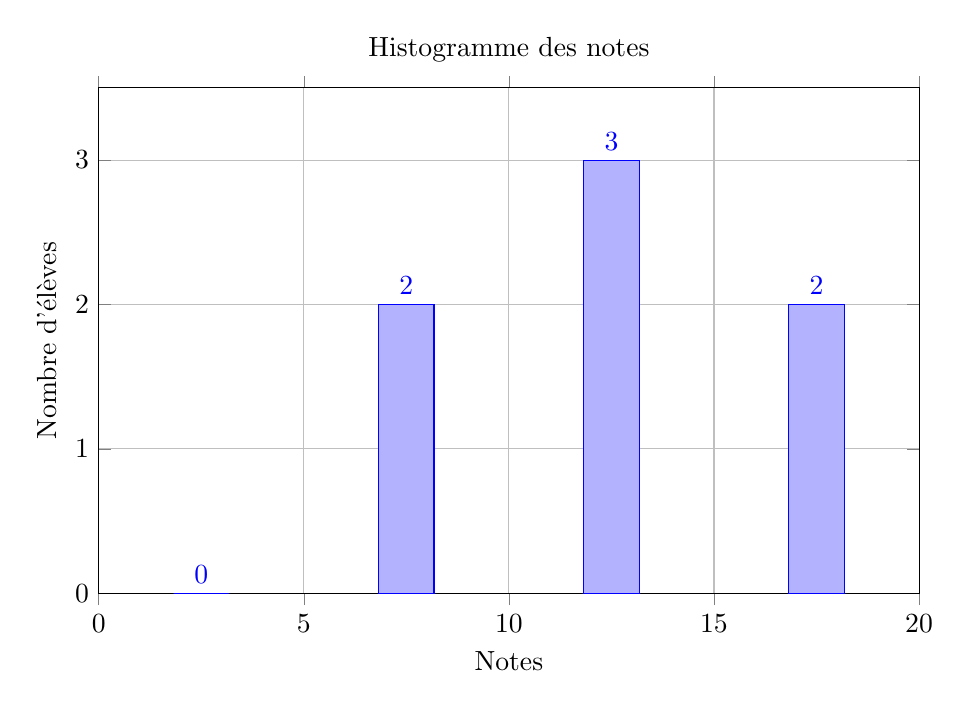
\begin{tikzpicture}
\begin{axis}[
    xlabel={Notes},
    ylabel={Nombre d'élèves},
    title={Histogramme des notes},
    ymin=0, ymax=3.5,
    xmin=0, xmax=20,
    width=12cm,
    height=8cm,
    xtick={0,5,10,15,20},
    ytick={0,1,2,3,4},
    grid=major,
    nodes near coords,
    nodes near coords align={vertical},
    ybar,
    bar width=20pt,
]
\addplot coordinates {(2.5,0) (7.5,2) (12.5,3) (17.5,2)};
\end{axis}
\end{tikzpicture}
\end{center}

\subsection{Répartition des Notes par Intervalles}

\begin{center}
\begin{tabular}{|l|c|c|}
\hline
\textbf{Intervalle de notes} & \textbf{Nombre d'élèves} & \textbf{Pourcentage} \\
\hline
{[}0 - 5{[} & 0 & 0,00\% \\
{[}5 - 10{[} & 2 & 28,57\% \\
{[}10 - 15{[} & 3 & 42,86\% \\
{[}15 - 20{]} & 2 & 28,57\% \\
\hline
\end{tabular}
\end{center}

\begin{center}
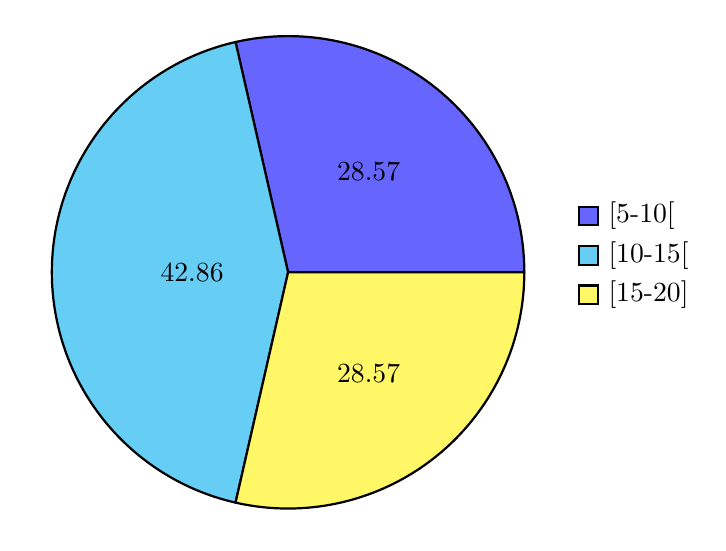
\begin{tikzpicture}
\pie[radius=3, text=legend, sum=auto]{28.57/{[5-10[}, 42.86/{[10-15[}, 28.57/{[15-20]}}
\end{tikzpicture}
\end{center}

\subsection{Taux de Réussite}
\begin{itemize}
\item Taux de réussite (note $\geq$ 10/20): 71,43\% (5 élèves)
\item Taux d'échec (note $<$ 10/20): 28,57\% (2 élèves)
\end{itemize}

\begin{center}
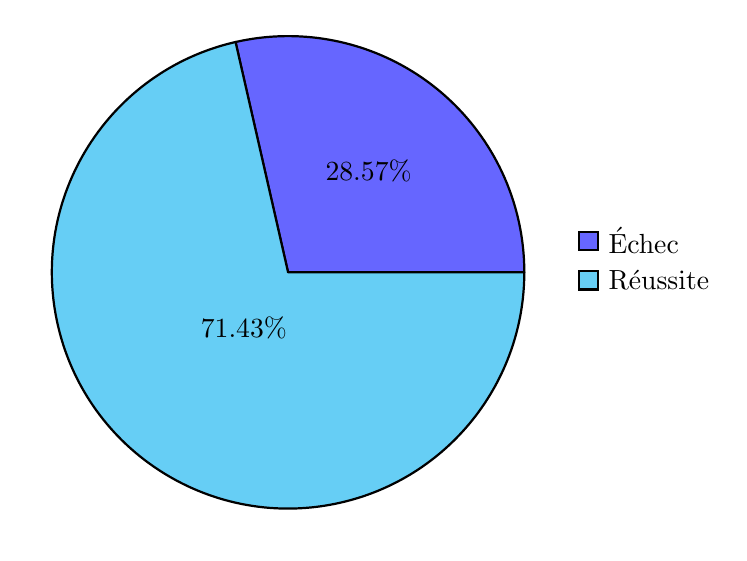
\begin{tikzpicture}
\pie[radius=3, text=legend]{28.57/Échec, 71.43/Réussite}
\end{tikzpicture}
\end{center}

\section{Analyse par Partie du Devoir}

\subsection{Performance Comparative Chimie/Physique}
En normalisant les résultats sur une base de 10 points pour faciliter la comparaison:

\begin{center}
\begin{tabular}{|l|c|c|}
\hline
\textbf{Partie} & \textbf{Moyenne /10} & \textbf{Taux de réussite} \\
\hline
Chimie (7 pts) & 5,86 /10 & 67,14\% \\
Physique (13 pts) & 6,05 /10 & 73,85\% \\
\hline
\end{tabular}
\end{center}

\begin{center}
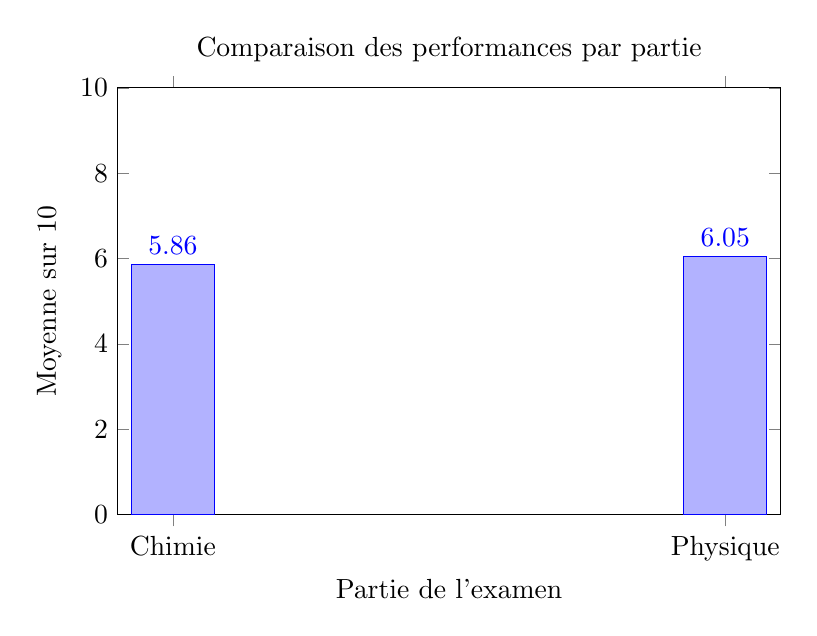
\begin{tikzpicture}
\begin{axis}[
    ybar,
    bar width=30pt,
    xlabel={Partie de l'examen},
    ylabel={Moyenne sur 10},
    title={Comparaison des performances par partie},
    symbolic x coords={Chimie, Physique},
    xtick=data,
    nodes near coords,
    nodes near coords align={vertical},
    ymin=0, ymax=10,
    width=10cm,
    height=7cm,
]
\addplot coordinates {(Chimie, 5.86) (Physique, 6.05)};
\end{axis}
\end{tikzpicture}
\end{center}

\subsection{Analyse par Compétence}

\begin{center}
\begin{tabular}{|l|c|}
\hline
\textbf{Niveau d'habileté} & \textbf{Performance moyenne} \\
\hline
Restitution des Connaissances & 71,25\% \\
Application des Connaissances & 64,38\% \\
Situation Problème & 55,71\% \\
\hline
\end{tabular}
\end{center}

\begin{center}
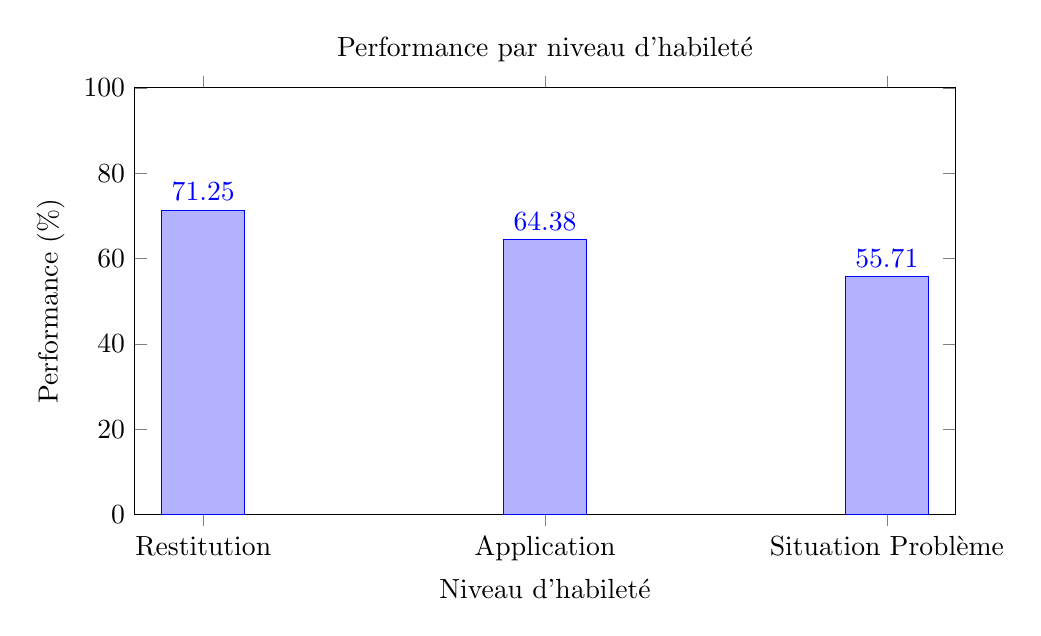
\begin{tikzpicture}
\begin{axis}[
    ybar,
    bar width=30pt,
    xlabel={Niveau d'habileté},
    ylabel={Performance (\%)},
    title={Performance par niveau d'habileté},
    symbolic x coords={Restitution, Application, {Situation Problème}},
    xtick=data,
    nodes near coords,
    nodes near coords align={vertical},
    ymin=0, ymax=100,
    width=12cm,
    height=7cm,
]
\addplot coordinates {(Restitution, 71.25) (Application, 64.38) ({Situation Problème}, 55.71)};
\end{axis}
\end{tikzpicture}
\end{center}

\section{Conclusion}

L’analyse des résultats du Devoir Surveillé N°1 met en évidence un taux de réussite satisfaisant de 71,43 \%, accompagné d’une moyenne de classe de 11,64/20, nettement supérieure à celle observée dans d’autres classes.

Les performances des élèves sont équilibrées entre les parties chimie et physique, avec un léger avantage pour cette dernière. Ils démontrent une bonne maîtrise des connaissances fondamentales, bien que certaines difficultés persistent face aux situations-problèmes complexes. Les axes d’amélioration concernent principalement l’interprétation physique des relations mathématiques et l’application des concepts dans divers contextes.

La progression positive par rapport aux autres classes peut s’expliquer par un meilleur équilibre dans le tableau de spécification et une approche pédagogique adaptée aux spécificités des élèves. Il est essentiel de renforcer l’articulation entre théorie et pratique, tout en développant l’autonomie des élèves face aux situations-problèmes.

Enfin, la classe de Sciences Mathématiques s’est particulièrement distinguée par une motivation et un engagement exceptionnels, qui ne sauraient être comparés à ceux des autres classes. Cet investissement remarquable mérite d’être encouragé et valorisé afin de maintenir cette dynamique d’excellence.
\end{document}
